\documentclass[a4paper,12pt,oneside,openany,table,xcdraw]{article}

\usepackage{setspace}
\usepackage{multirow}
\usepackage{hyperref}
\usepackage{caption}
\usepackage{indentfirst}

\usepackage[brazilian]{babel}
\usepackage[utf8x]{inputenc}
\usepackage{amsmath, graphicx, enumerate}
\usepackage{float, verbatim}
\usepackage[colorinlistoftodos]{todonotes}
\usepackage{makeidx} % Para o sumário
\usepackage{geometry}

\geometry{a4paper, hmargin={3cm, 3cm}, vmargin={3cm, 2cm} }
\setlength{\parindent}{1.0cm}
\graphicspath{{img/}}

\begin{document}
\newcommand{\thedepartment}{Faculdade de Engenharia Elétrica}
\newcommand{\thecourse}{FEELT}
\newcommand{\thetitle}{FONTE DE ALIMENTAÇÃO LINEAR REGULADA}
\newcommand{\thetype}{Relatório da Disciplina de Eletrônica Analógica I}
\newcommand{\theproftitle}{Bacharel em Engenharia Elétrica}
\newcommand{\thestudent}{Ana Júlia Costa Santana \_ 
11811ETE003\\Lesly Viviane Montúfar Berrios \_ 
11811ETE001}
\newcommand{\theadvisor}{Prof. Daniel Pereira de Carvalho}
\newcommand{\thecity}{Uberlândia}

\thispagestyle{empty}\newcommand*{\themonth}{\ifthenelse{\the\month < 2}{Janeiro }
                  {\ifthenelse{\the\month < 3}{Fevereiro }
                  {\ifthenelse{\the\month < 4}{Março }
                  {\ifthenelse{\the\month < 5}{Abril }
                  {\ifthenelse{\the\month < 6}{Maio }
                  {\ifthenelse{\the\month < 7}{Junho }
                  {\ifthenelse{\the\month < 8}{Julho }
                  {\ifthenelse{\the\month < 9}{Agosto }
                  {\ifthenelse{\the\month < 10}{Setembro }
                  {\ifthenelse{\the\month < 11}{Outubro }
                  {\ifthenelse{\the\month < 12}{Novembro }{Dezembro }}}}}}}}}}}}
                  
\begin{titlepage}
\begin{center}

	\vspace{-0.5cm}

  \begin{figure}[hbt!]
		\begin{center}
		   
\includegraphics[width=2.8cm]{ufu-logo.png}
		\end{center}
	\end{figure}
 	%\vspace{-4cm}

%\begin{doublespacing}

  \Large{\textbf{Universidade Federal de Uberlândia}}\\
  \large{\thedepartment}\\
  \large{\thecourse}\\


\vspace{5.8cm}
  \par
  \large\textbf{\thetitle}
\vspace{5.8cm} 

%\end{doublespacing}
  \par
  \thetype\\
  por\\
  %\hspace{2cm}\large{}\\

\vspace{0.8cm}
\par
  \normalsize{\thestudent}\\ [2cm]
  \theadvisor

\par\vfill
  \thecity, \themonth / \the\year

\end{center}

\end{titlepage}

%% Comeca o documento !

\onehalfspacing
\tableofcontents % sumário
\newpage

\section{Introdução}
Um fonte de alimentação
trata-se de um dispositivo responsável por converter a tensão elétrica alternada e alta (gerada na tomada) para uma tensão menor e que pode ser alternada ou contínua, dependendo do aparelho eletrônico.
De forma geral, a finalidade das fontes é converter a energia e alimentar os aparelhos de maneira eficiente.
Basicamente, existem dois modelos de fontes de alimentação: a linear e a chaveada.

As fontes de alimentação lineares funcionam muito bem para aplicações de baixa potência, como os telefones sem fio, por exemplo. Entretanto, quando é necessário uma potência maior, as fontes lineares tendem a ser muito grandes para a tarefa. Isto porque, quanto menor a frequência de tensão alternada, maior o tamanho dos componentes. 

Sendo assim, estas fontes não são utilizadas para os computadores portáteis, pois seriam muito grandes e pesadas para poderem ser carregadas para todos os lugares. A solução para isso foi o uso do chaveamento em alta frequência, que deu origem as fontes chaveadas.

Em fontes de alimentação chaveadas em alta frequência, a tensão de entrada tem sua frequência aumentada antes de ir para o transformador. Com a frequência maior, o transformador e os capacitores eletrolíticos podem ser bem menores. 
É este tipo de fonte que é utilizada para os computadores e para muitos outros equipamentos eletrônicos menores. O termo “chaveada” se refere ao chaveamento de alta frequência, não tendo ligação com a fonte ter uma chave de liga/desliga \cite{hayama}.

% A importancia da fonte

\newpage
\section{Planejamento} % e simulações
A seguir estão dispostas as primeiras considerações para a realização do projeto, desde a análise do circuito base por meio de simulações, até à escolha dos componentes a serem utilizados na confecção do circuito impresso.

\subsection{Circuito esquemático}
A Figura \ref{circuito} mostra o circuito no qual este projeto se baseia, extraída de \cite{amp}. Ademais, para melhor comprenssão do circuito tem-se o esquemático em \ref{sim1}, do qual é posssível obter dados de simulação. Vale ressaltar que a explicação prévia do professor foi importante para melhor entendimento do procedimento a ser realizado, sendo na Figura \ref{quadro} comtemplado parte de sua explanação.

\begin{figure}[H]
\centering
\captionsetup{font=scriptsize}
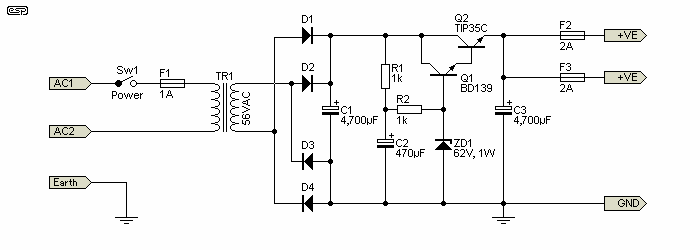
\includegraphics[width=16cm]{fonte}
\caption{Circuito da fonte de alimentação \cite{amp}.}
\label{circuito}
\end{figure}

\begin{figure}[H]
\centering
\captionsetup{font=scriptsize}
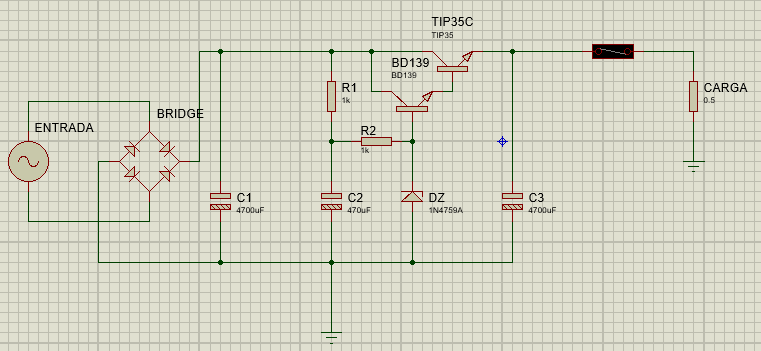
\includegraphics[width=16cm]{sim1}
\caption{Circuito da fonte de alimentação em MULTSIM.}
\label{sim1}
\end{figure}

\begin{figure}[H]
\centering
\captionsetup{font=scriptsize}
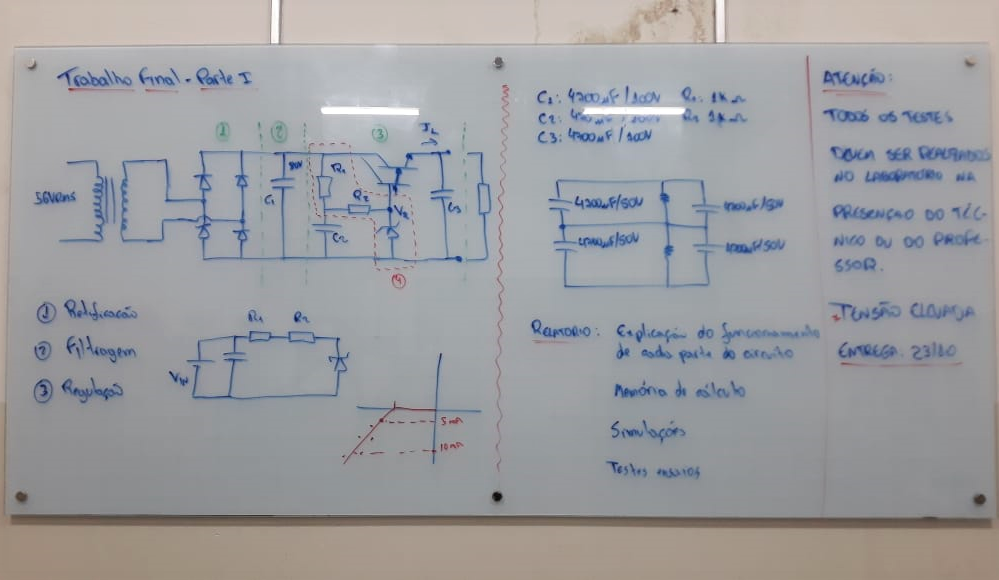
\includegraphics[width=16cm]{quadro}
\caption{Explicação prévia em sala de aula.}
\label{quadro}
\end{figure}

\subsection{Componentes}
\begin{enumerate}[1 -]
    \item \textbf{\emph{Ponte retificadora:}} Optou-se pela ponte retificadora GBJ606, pois possui corrente máxima de 6A.
    \item \textbf{\emph{Capacitores:}} De acordo com a disponbilidade de capacitores nos principais pontos de venda de eletrônicos em Uberlândia, conseguiu-se dois capacitores de $4700\mu F$ - 100V e um capacitor de $470\mu F$ - 200V.
    \item \textbf{\emph{Resistores:}} Foram utilizados dois resistores de 1K para re
    \item \textbf{\emph{Diodo Zener:}}
    \item \textbf{\emph{Transistores:}}
    \item \textbf{\emph{Fusíveis:}}

    
    
\end{enumerate}

\subsection{Sobre o projeto}
 
   Ao projetar uma fonte  de forma  eficiente, alguns cuidados são necessários. Tendo como base o projeto original, alguns ajustes foram realizados para modernizá-lo, como a substituição dos diodos e a sua constituição, trocando o germânio pelo silício, e os modelos de transistor utilizados. Seguindo as orientações do professor, também foram acrescentados alguns componentes.
   
   Além disso, devido a mudanças realizadas no circuito, a etapa de simulação  do circuito é essencial, para verificar seu funcionamento, antes da montagem. Assim, é ideal que uma nova análise matemática seja realizada a fim de verificar o funcionamento da fonte com parâmetros reais, já que na engenharia quase nenhum processo é exato e depende de fatores ambientais e humanos.
 
\subsection{Orçamento}

Para realizar a construção da fonte, vários componentes foram necessarios, a maioria desses sendo adquirida no centrida no Centro  Eletronico , com exceção dos capacitores de 4700 uF , ambos aquisicionados em diferentes lojas em Uberlândia , além do diodo Zener.
Todas as despesas totalizam , oq eu se encontra dentro do orçamento simulado pelo professor durante a primeira  as primeiras orientações para o projeto.

\newpage
\section{Simulação}
Para a realização de cada etapa foi essencial a verificação de tensão e correntes máximas sobre os componentes a fim de evitar um curto-circuito.
Por exemplo, antes de realizar a compra dos capacitores foi necessária a verificação da tensão máxima que este deveria suportar, a qual observa-se na Figura \ref{sim2}. Assim, verificou-se que seriam necessários capacitores que suportassem 80V ou mais, porém devido à disponibilidade escassa de capacitores na medida à risca, optou-se por dois capacitores 100V ($4700\mu F$) e um, 200V ($470\mu F$). Note que, já que a fonte não possui carga conectada, foi suposota uma carga de valor baixo de $0,5 \Omega$.

\begin{figure}[H]
\centering
\captionsetup{font=scriptsize}
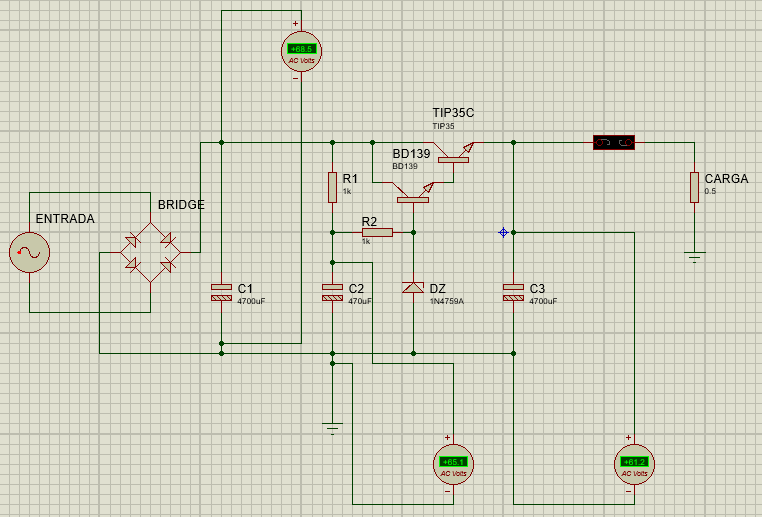
\includegraphics[width=16cm]{sim2}
\caption{Tensões máximas sobre os capacitores.}
\label{sim2}
\end{figure}

\newpage
\section{Funcionamento do circuito}
A tensão de entrada é primeiramente rebaixada de $220V/127V$ para $56V$ com auxílio do regulador de tensão (também chamado de \emph{varivolt}). Assim, obter-se-á uma tensão senoidal de menor amplitude que ainda será convertida em contínua com intuito de ser utilizada para alimentar o amplificador.

\subsection{Retificação}
Esta etapa transforma a tensão alternada em uma tensão contínua pulsa ante
, e é realizada principalmente pela ponte retificadora. a ponte escolhida foi uma de 6A, 100 V que atende aos parâmetros do  circuito montado.
\subsection{Filtragem}
transforma a tensão contínua pulsante em uma tensão contínua quase perfeita. Mas essa tensão contínua apresenta, quando a fonte é ligada a uma carga, uma oscilação chamada Tensão de Ripple. Essa etapa é realizada pelos capacitores encontrados eno circuito que devido a sua composição, ao sofrer o processo de carga e descarga diminuem a oscilação da tensão já que a tensão fornecida ao circuito agora nos momentos de pulso é suprida pela descarga do capacitor. Porém como abprdado anteriormente, resta ainda o riplle e para eliminar esse fator incômodo existe ainda outra etapa...

\subsection{Regulação}
Esta última etapa tem por objetivo eliminar por completo a tensão de oscilação.  É cla,7 que não elimina totalmente, mas remove boa parte. Esta última etapa pode consistir em regulação com diodo zener, com emissor zener, existem também alguns circuitos com transistores e, por último, reguladores em CI, como a família 78XX para tensões positivas e 79XX para tensões negativas.

\newpage
\section{Memória de Cálculo}

\subsection{Espessura da linha}

Ao projetar a plca de circuito impresso. Um cuidado maior com relação as trilhas precisa ser tomado, para que não haja problemas quanto a passagem de corrente, e para otimizar a dissipção do calor na placa. 
Para escolher uma espessura de linha que cumprisse tais propósitos utilizamos o equacionamento de acordo com a norma IPC-2221, que através de sua curva define as constantes k, b e c que são utilizadas no cálculo da espessura da trilha mais adequada.
Iniciando pelo cálculo da Área temos:

\begin{math}
A [\mathit{th^{2}}] = (I/ (k * (Temp-Rise [deg. C])^{b}))^{\frac{1}{c}}
 \end{math}
 
E em sequência a largura é dada:
\begin{math}
L [\mathit{th}] = (A/(Espessura [oz] * 1,378)
 \end{math}

Considerando  k = 0,048, b = 0,44, c = 0,725 e a placa de fenolite de 1 OZ, e uma variação de temperatura de aproximadamente \begin{math} 10^{\circ}C  \end{math} , descobriu-se um valor para a espessura das linhas de aproximadamente 90 th. Que foi o tamanho utilizado em quase toda a placa projetada.


\subsection{Resistor de Descarga}

Para segurança do circuito,e daqueles que forem manejá-lo, resistores foram acrescentados em paralelo com os capacitores, para que, ao efetuar o desligamento da placa os capacitores pudessem ser descarregados em segurança.
Para projetar a resistência necessária nos capacitores, as equações conhecidas para descarga num capacitor foram aplicadas.

\begin{math} t= RCln\left ( 1 - \frac{V_{C}}{V_{in}} \right ) \end{math}

Considerndo os capacitores de 4700uF e um tempo de descarga de 10 s, para uma tensão média entre os dois capacitores, \begin{math}V_{C}\end{math} de 64,85 V (de acordo com simulação) e \begin{math}V_{in}\end{math} de 80 \begin{math}V_{pp}\end{math}, a resitência mínima necessária é de 1,3 K\begin{math}\Omega\end{math}, para suprir esses requisitos mínimos, foi utilizado um reistor de 1,8 K\begin{math}\Omega\end{math} de 5W. 


\subsection{Regulação}

Regualação para 62 V, PARAMETROS DO DIODO ZENER.

De linha e de carga.

\section{Testes e ensaios}
Não foi possível ainda a realização desta etapa, devido a diversos imprevistos e falta de organização.


\newpage
\begin{thebibliography}{9} 

\bibitem{hayama}
    Hayama,
    “Fontes de alimentação – O que são, para que servem e quais são os modelos?”, Hayama.
 Disponível em:
 \url{blog.hayama.com.br/fontes-de-alimentacao/}. Acesso em: out. 2019.

\bibitem{amp}
    Rod Elliott,
    “El Cheapo - A Really Simple Power Amplifier”, ESP, Elliott Sound Products, 2005.
 Disponível em:
 \url{https://sound-au.com/project12a.htm}. Acesso em: out. 2019.
 
 \bibitem{espess}
    Brooks Doug,Graves Dave,
    "Current Carrying Capacity of Vias"
 Disponível em : 
 \url{https://www.ultracad.com/articles/viacurrents.pdf}. Acesso em : out. 2019.
 
 \bibitem{res}
    Soares Camila,
 "Dedução das equações de carga e descarga dos capacitores utilizando equações diferenciais de primeira ordem"
  Disponível em : 
 \url{https://camilasoares.wordpress.com/2009/04/07/deducao-das-equacoes-de-carga-e-descarga-dos-capacitores-utilizando-equacoes-diferenciais-de-primeira-ordem/}.
 Acesso em : out. 2019.
 
 \bibitem{comp}
    Petry Clovis Antonio,
 "D. PROJETO DE PLACAS DE CIRCUITO
IMPRESSO - BÁSICO "
  Disponível em : 
 \url{http://www.professorpetry.com.br/Bases_Dados/Apostilas_Tutoriais/Projeto_PCI_Charles.pdf}. Acesso em : out. 2019.
 
 % DATASHEETS
 
 \bibitem{GBJ606} % ponte retificadora
        “6.0A GLASS PASSIVATED BRIDGE RECTIFIER
”, DIODES INCORPORATED.
 Disponível em:
 \url{https://www.diodes.com/assets/Datasheets/ds21216.pdf}. Acesso em: out. 2019.
 
  \bibitem{DB139} % transistor
    “BD135/137/139
”, FAIRCHILD SEMICONDUCTOR.
 Disponível em:
 \url{http://www.redrok.com/NPN_BD135_45V_1.5A_12.5W_Hfe40_TO-126.pdf}. Acesso em: out. 2019.
 
 \bibitem{TIP35} % transistor
    “Silicon NPN Power Transistors TIP35/35A/35B/35C ”, SavantIC Semiconductor. 
 Disponível em:
 \url{https://pdf1.alldatasheet.com/datasheet-pdf/view/269985/SAVANTIC/TIP35.html}. Acesso em: out. 2019.
 


\end{thebibliography}
\end{document}
